\documentclass[a4paper]{report}

\usepackage[utf8]{inputenc}
\usepackage[T1]{fontenc}
\usepackage{hyperref}
\usepackage[francais]{babel}
\usepackage{hyperref}
\usepackage{graphicx}

\title{Rubik'INT \\ Livrable 1}
\author{Rémy \bsc{ZIRNHELD} \and Alban \bsc{MANZANO} \and Florian \bsc{GRANTE} \and Nicolas {BONNET}}
\date{7 février 2017}

\begin{document}

\maketitle

\tableofcontents

\chapter*{Introduction}
\addcontentsline{toc}{chapter}{Introduction}

Le projet de développement informatique nous a offert l'opportunité de créer le programme que nous voulions.
Divers sujets se présentaient à nous. Nous étions déterminés à trouver un projet nous permettant de mettre en œuvre plusieurs domaines de l'informatique.
Nous avons choisi le Rubik's Cube, un casse-tête fascinant: il s'agit d'un cube constitué de 3x3x3 sous-cubes colorés pouvant tourner selon trois axes.
Le Rubik's Cube se distingue par l'immense complexité de sa résolution contrastant avec sa simplicité apparente.
Chaque personne capable de résoudre le cube doit suivre une méthodologie stricte et faire preuve d'une certaine intuition.
L'objectif derrière le choix de ce célèbre casse-tête en tant que sujet est d'apprendre des domaines de l'informatique qui sont nouveau pour nous.

Le défi que nous nous sommes lancé est d'apprendre à une machine à résoudre ce casse-tête.
Pour cela nous devrons nous confronter à plusieurs problématiques.
La première, la plus évidente, est sa résolution. Nous allons avoir besoin de faire appel à des connaissances mathématiques et algorithmiques.
De plus nous voulons donner un aspect pratique à notre projet. Ainsi, l'utilisateur devra pouvoir réussir à résoudre son cube grâce au programme.
Il est donc indispensable d'élaborer une interface utilisateur.
Nous devrons aussi ajouter une solution simple pour reconnaitre la configuration du cube dans le programme. Nous utiliserons un algorithme de \textit{computer vision} sur un flux vidéo acquis en temps réel par une webcam.
Ainsi, ce projet regroupe les thématiques du traitement d'image, de l'algorithmie et du traitement d'image.

\chapter{Cahier des charges}
\section{Premier prototype}
Il s'agit premièrement d'implémenter la fonction basique de notre programme: la résolution du cube. Nous allons donc lui fournir en entrée un fichier contenant les couleurs de toutes les facettes du cube. Le programme cherchera à le résoudre et renverra les mouvements nécessaires à sa résolution. Par exemple en utilisant la notation de Singmaster\footnote{Plus d'information sur cette notation: \url{https://ruwix.com/the-rubiks-cube/notation/}}.
Différentes méthodes sont pour l'instant envisagées:
    -La première consiste à implémenter l'algorithme de résolution simple appris en général en premier par les humains. Elle consiste à envisager la résolution dans l'ordre suivant: d'abord une face, puis la première et seconde couronne et enfin la dernière face. \footnote {voir \url{https://www.francocube.com/cyril/rubik_index}} Pour résoudre le rubik's cube de cette manière, le programme devra être capable de reconnaitre la configuration dans laquelle se trouve le cube à un moment donné et lui
    appliquer une procédure, c'est-à-dire une suite prédéfinie de rotations. Les autres méthodes utilisées par les humains reposent sur ce même principe avec différentes configurations et procédures. Dans le cas des méthodes dites avancées, c'est-à-dire permettant de résoudre le Rubik's cube en un nombre plus petit de rotations, le nombre de configurations et de procédures à apprendre augmente drastiquement.
	-Un algorithme reposant sur une machine de boltzmann est également envisagée. Cet algorithme aurait une fonction d'évaluation de l'énergie du cube (plus le cube est proche de sa résolution, plus son énergie est faible) et chercherait à minimiser cette énergie via des rotations aléatoires ou des procédures aléatoires. Ces procédures auraient d'autant plus de chances d'être choisie que leur action réduit l'énergie du cube. Cet algorithme pourrait être utilisé conjointement avec le premier pour la résolution.
	-Un troisième algorithme dit en deux phases consiste à utiliser un algorithme A* (parcours d'un arbre en profondeur amélioré par un heuristique) pour placer les angles du cube au bon endroit lors de la première phase. La seconde phase consiste à utiliser réduire le nombre de rotation possible à un groupe de cardinal plus petit. Cet algorithme permet de résoudre le Rubik's Cube en une vingtaine de coups, mais est également plus dur à implémenter.

\section{L'affichage en 3D}
La prochaine étape du développement consiste à faire une interface homme machine. Il faut que l'utilisateur puisse visualiser les étapes successives de résolution du Rubik's Cube. Pour cela nous comptons afficher une fenêtre avec un bouton pour aller à l'étape suivante et une image en 3D de la configuration du cube que l'utilisateur devrait avoir dans les mains.

\section{\textit{Computer vision}}
Une fois que l'affichage a été réalisé, il faut pouvoir permettre de rentrer la configuration du cube au départ. Pour cela nous présenterons les différentes faces du cube à la caméra et un algorithme de traitement d'image sera capable de reconstituer le cube virtuellement.

\chapter{Interface}
Nos recherches sur la façon de réaliser un rendu 3D en java nous à amener sur une librairie : \textit{Java3D} . Même si le rendu à un instant t est satisfaisant (voir image ci-dessous), il ne nous permet pas, du moins de façon optimisé, de réaliser des animations comme la rotation du cube car le rendu est figé une fois affiché.
\begin{center}
	\makebox[\textwidth]{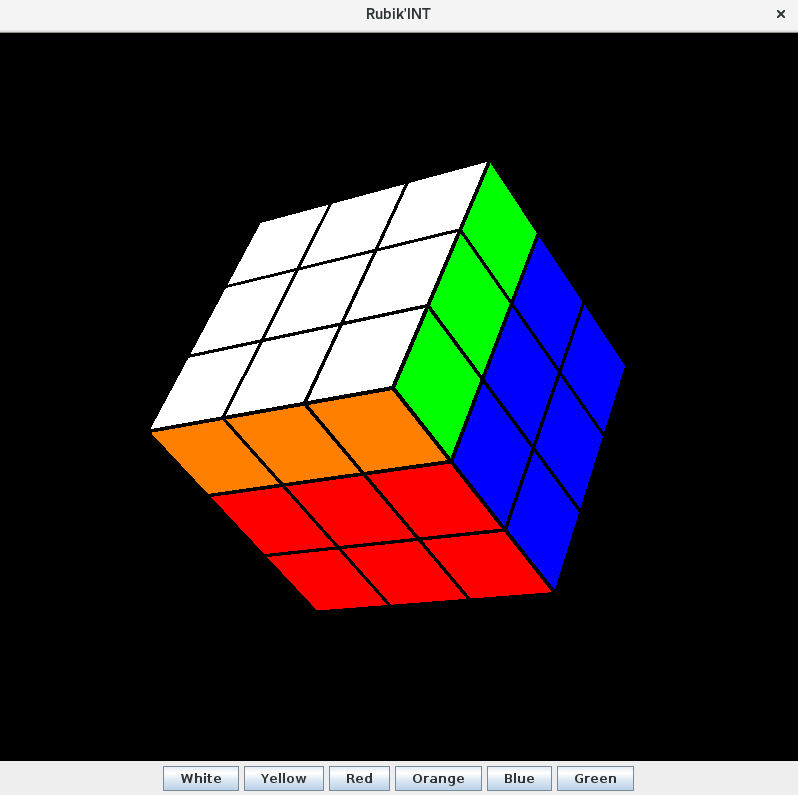
\includegraphics[width=.8\paperwidth]{diagramme/rendu3D.png}}
\end{center}
Cet essaie nous à permis de mieux cerner notre besoin, c'est à dire un rendu 3D où l'objet affiché reste modifiable, ici notre cube, et donc de pouvoir réaliser les animation de rotation de ce dernier. C'est pourquoi nous avons finalement décider de réaliser tout cela à l'aide d'une librairie bien connue : \textit{OpenGL}

Maintenant que notre besoin technique vis à vis de l'affichage 3D est définie, il devra être intégré dans une interface, ie accompagné de boutons pour rendre notre programme de résolution autonome et facile d'utilisation. Nous pouvons voir une ébauche d'utilisation de la librairie \textit{Swing} sur la photo ci-dessus. L'objectif de cette première fenêtre est de faire tourner la face du cube de la couleur associé au bouton lorsque l'utilisateur clique dessus.

A terme, l'interface sera scindé en trois parties selon la logique suivante :

	-Un accueil pour que l'utilisateur puisse choisir la façon dont il veut résoudre son Rubik's cube (Avec ou sans prise de photo d'un vrai cube)
	-Une interface permettant la prise de photo du cube et donc de récupérer sa configuration pour qu'il puisse ensuite passer à sa résolution
	-Une interface pour la résolution du cube.

De cette façon notre programme est clairement défini ce qui le rend plus "user friendly".


\chapter{Structure du code}

Maintenant que les besoins ont étés traîtés, il convient de s'intéresser à la façon dont nous allons organiser notre code. Puisque nous avons choisi Java comme langage de programmation, la conception du programme se fera sous la lumière de la programmation orientée object. Nous allons donc maintenant définir les classes dont nous allons avoir besoin pour notre projet.

\paragraph{Le Rubik's cube} Premièrement, notre programme manipule un Rubik's cube. Il s'agit donc de définir l'organisation de ces objets:

\begin{center}
      \makebox[\textwidth]{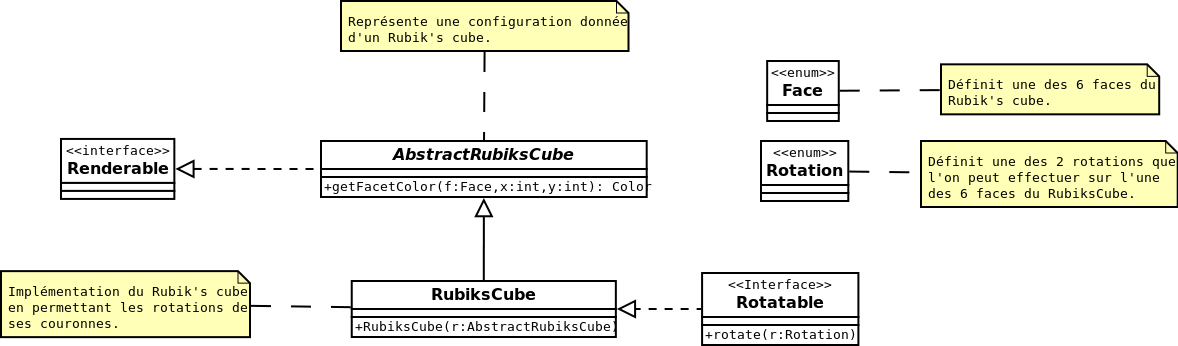
\includegraphics[width=.8\paperwidth]{diagrammes/rubikscube.png}}
\end{center}
Ainsi \textit{AbstractRubiksCube} servira lorsque que nous aurons besoin d'informations sur une configuration donnée du Rubik's Cube alors que \textit{RubiksCube} permettra la manipulation de cet objet via l'interface \textit{Rotatable}. 


\paragraph{Rubik'Int} Notre application - donc notre classe principale - sera appelée RubikInt. Elle aura pour rôle de commander les autres objets pour que le programme ait le comportement désiré. Ainsi on peut dessiner un diagramme montrant ses interactions avec les différents autres objets:

\begin{center}
      \makebox[\textwidth]{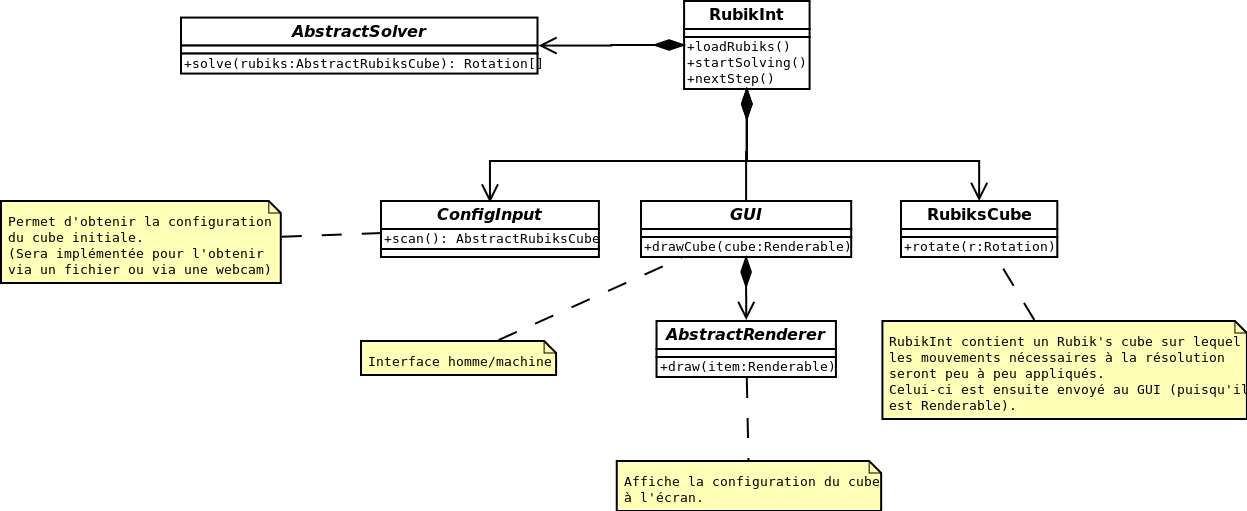
\includegraphics[width=.8\paperwidth]{diagrammes/projet.png}}
\end{center}
Ainsi on voit ressortir les différents point importants de notre projet: 
\begin{itemize}
    \item L'interface homme/machine, qui se caractérise par l'implémentation de des classes \textit{GUI} et \textit{AbstractRenderer}.
    \item L'algorithme de résolution qui devra être mis en place dans l'implémentation de \textit{AbstractSolver}. Plusieurs variantes pourront êtres mises en oeuvre.
    \item La structure de donnée choisie pour représenter le Rubik's Cube, dans sa classe \textit{RubiksCube}.
    \item L'interface permettant de rentrer la configuration d'un Rubik's Cube dans \textit{ConfigInput}. Nous pourrons par exemple charger cette configuration d'un fichier, laisser l'utilisateur la rentrer sur une interface graphique ou même l'obtenir via une caméra.
\end{itemize}


\chapter*{Conclusion}
\addcontentsline{toc}{chapter}{Conclusion}

\end{document}
